In previous work~\cite{deligiannis2015psharp}, we approached the problem of testing legacy distributed systems as follows. First, we ported the system to \psharp, we then modeled its environment as \psharp state machines, and then we tested the ported system and its environmental model using the \psharp systematic concurrency testing engine. The limitation of this approach is that it does not allow us to directly test a legacy system, as it has to be re-implemented first in \psharp. However, such endeavor is very costly and time consuming, and thus is not realistic for testing an existing production system, such as the Azure Storage vNext.

In order to solve this problem, and allow \psharp to be used for testing \emph{unmodified} legacy distributed systems, we decided to take a radically different modeling approach. Our approach is \emph{flexible}, involves the use of \emph{simple language features} that developers already use for testing their systems, and can be applied to production code.

We only model the environment of the program that we would like to test, and then allow the developer to connect the original system with the environmental model using \emph{dynamic dispatch}, which is provided by the \csharp runtime.

We now give an example of using dynamic dispatch to model the network engine of the extent manager in the Azure Storage vNext case study.

\begin{figure}[t]
\centering
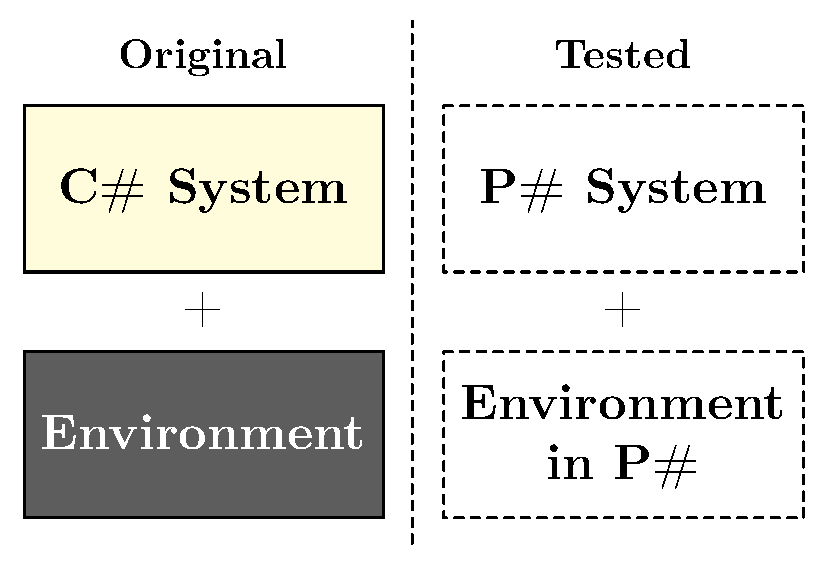
\includegraphics[width=\linewidth]{img/models_old}
\caption{Draft.}
\label{fig:oldapproach}
\end{figure}

\begin{figure}[t]
\centering
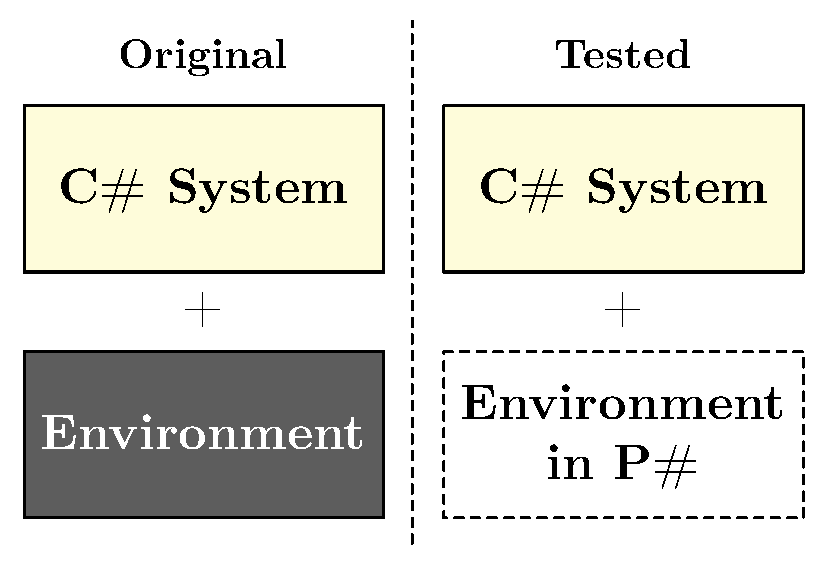
\includegraphics[width=\linewidth]{img/models_new}
\caption{Draft.}
\label{fig:newapproach}
\end{figure}

\PDComment{mention dependency injection pattern?}
